% !TEX root = ../main.tex

\section{实验设置}
\label{sec:metartl-setup}

\subsection{数据集、任务与评价指标}

实验采用 SJTUTables 和 RelBench 两组公开关系表格数据
\cite{li2024rllm,robinson2024relbench}。
SJTUTables 包含 TACM12k、TLF2K 和 TML1M 三个多分类任务，
采用准确率评价；RelBench 包含七个数据库上的十二个
二分类任务和九个回归任务，分别采用 ROC-AUC 和平均绝对误差（MAE）
评价。两组数据共包含十个数据库、二十四项任务。
表~\ref{tab:metartl-datasets} 列出数据集规模和各数据集的关系跳数统计值；
候选元路径长度上限统一设置为四跳。

\begin{table}[htbp]
  \centering
  \caption{实验数据集规模}
  \label{tab:metartl-datasets}
  \begin{tabular}{lrrrr}
    \toprule
    数据集 & 表数 & 总行数 & 列数 & 统计表最大跳数 \\
    \midrule
    TACM12k    & 4  & 97,774     & 12  & 2 \\
    TLF2K      & 3  & 101,773    & 15  & 1 \\
    TML1M      & 3  & 1,010,132  & 20  & 2 \\
    rel-f1     & 9  & 97,606     & 77  & 3 \\
    rel-trial  & 15 & 5,852,157  & 140 & 3 \\
    rel-avito  & 8  & 20,679,117 & 43  & 2 \\
    rel-amazon & 3  & 24,291,489 & 15  & 2 \\
    rel-hm     & 3  & 33,265,846 & 37  & 2 \\
    rel-stack  & 7  & 38,109,828 & 51  & 3 \\
    rel-event  & 5  & 41,328,337 & 128 & 2 \\
    \bottomrule
  \end{tabular}
\end{table}

\subsection{对照方法与实现设置}

单表对照包括梯度提升树 LightGBM\cite{ke2017lightgbm}，以及
FTTransformer\cite{gorishniy2021tabular}、
Trompt\cite{chen2023trompt} 和
ExcelFormer\cite{chen2024excelformer} 三种表格深度学习模型。
多表对照包括 RelBench 中的 RDL、BRIDGE、RelGNN 和 LightRDL；
它们分别代表基于表格编码器和异构 GraphSAGE 的方法、使用受限辅助表
的图方法、复合关系消息传递方法以及利用预训练表格模型的方法
\cite{fey2024rdl,li2024rllm,chen2025relgnn,lachi2025lightrdl}。
单表方法通过连接目标表与对应特征表构造输入。
在包含多个辅助实体表的任务中，BRIDGE 使用与目标表最相关的一个辅助表。
RelGNN 与 LightRDL 根据其发布代码和论文描述复现；
对于缺少时间字段的 SJTUTables 数据，LightRDL 使用生成的时间戳。
这些设置构成相应方法在本实验中的实现条件。

MetaRTL 的预训练阶段进行五个训练轮次。模型采用四层、隐藏维度为
128 的表格编码器，两层、隐藏维度均为 128 的异构图网络，
候选元路径最长四跳，跨批共享原型数为 4096。表格编码器采用
ResNet 风格模块，异构图网络采用 GraphSAGE 风格模块。
RelBench 任务采用时间感知的均匀邻域采样，并遵循基准数据集的
任务划分及评价协议。

\section{预测性能比较}
\label{sec:metartl-results}

\subsection{SJTUTables 多分类任务}

表~\ref{tab:metartl-sjtu} 给出三个 SJTUTables 任务的准确率。
MetaRTL 在三项任务中均为表内最高：TACM12k 为 $46.54\%$，
TLF2K 为 $43.17\%$，TML1M 为 $37.09\%$。
其中 TACM12k 相对表内最佳单表方法 LightGBM 高
$10.84$ 个百分点；TLF2K 和 TML1M 相对各自最强的
其他多表方法 BRIDGE 分别高 $0.97$ 和 $0.89$ 个百分点。
三项任务的提升幅度存在差异，表明模型收益与数据集特征及任务有关。

\begin{table}[htbp]
  \centering
  \caption{SJTUTables 多分类任务的准确率（\%，越高越好）}
  \label{tab:metartl-sjtu}
  \begin{tabular}{lrrr}
    \toprule
    方法 & TACM12k & TLF2K & TML1M \\
    \midrule
    LightGBM     & 35.70 & 35.52 & 26.66 \\
    FTTransformer & 14.88 & 15.80 & 28.62 \\
    Trompt       & 12.42 & 13.41 & 27.85 \\
    ExcelFormer  & 17.13 & 20.61 & 31.90 \\
    RDL          & 19.23 & 19.58 & 26.93 \\
    RelGNN       & 18.19 & 20.31 & 27.12 \\
    BRIDGE       & 25.60 & 42.20 & 36.20 \\
    LightRDL     & 24.94 & 39.17 & 35.77 \\
    \textbf{MetaRTL} & \textbf{46.54} & \textbf{43.17} & \textbf{37.09} \\
    \bottomrule
  \end{tabular}
\end{table}

\subsection{RelBench 分类与回归任务}

表~\ref{tab:metartl-relbench-cls} 和表~\ref{tab:metartl-relbench-reg}
给出二十一项 RelBench 任务的预测结果。
为节约版面，表头中 FT、Excel、RGNN、BR 和 L-RDL
分别表示 FTTransformer、ExcelFormer、RelGNN、BRIDGE 和 LightRDL。
MetaRTL 在十二个分类任务中的九个取得单独最高 ROC-AUC，
在 \texttt{user-badge} 上与 RelGNN 并列最高；在九个回归任务中的
八个取得最低 MAE。综合来看，二十一项任务中有十七项单独最优、
一项并列最优，另有三项未达到最优。分类和回归任务的平均名次
分别为 $1.33$ 和 $1.67$。

\begin{table}[p]
  \centering
  \caption{RelBench 二分类任务的 ROC-AUC（越高越好）}
  \label{tab:metartl-relbench-cls}
  \resizebox{\textwidth}{!}{%
  \begin{tabular}{llrrrrrrrrr}
    \toprule
    数据集 & 任务 & LightGBM & FT & Trompt & Excel & RDL & RGNN & BR & L-RDL & MetaRTL \\
    \midrule
    rel-f1 & driver-top3       & .7392 & .7362 & .7317 & .7522 & .7723 & .8086 & .7713 & .7916 & .8415 \\
           & driver-dnf        & .6856 & .6831 & .6752 & .6720 & .7125 & .6706 & .7016 & .6863 & .7418 \\
    rel-trial & study-outcome   & .7009 & .6239 & .6573 & .6731 & .6902 & .6916 & .6898 & .6815 & .7013 \\
    rel-avito & user-clicks     & .5360 & .5132 & .5423 & .5532 & .6576 & .6613 & .5501 & .6411 & .6614 \\
              & user-visits    & .5305 & .5210 & .5611 & .5501 & .6599 & .6547 & .5616 & .6239 & .6587 \\
    rel-amazon & user-churn     & .5222 & .5230 & .5310 & .5209 & .7042 & .6544 & .5351 & .6917 & .7101 \\
               & item-churn    & .6254 & .6415 & .5982 & .6250 & .8281 & .8264 & .6993 & .8120 & .8290 \\
    rel-hm & user-churn        & .5521 & .5013 & .5419 & .5395 & .7011 & .6810 & .5933 & .6713 & .6795 \\
    rel-stack & user-engagement & .6339 & .6002 & .6573 & .6920 & .9047 & .8995 & .7974 & .8902 & .9120 \\
              & user-badge     & .6343 & .6036 & .6282 & .6713 & .8886 & .8898 & .8790 & .8671 & .8898 \\
    rel-event & user-repeat    & .6804 & .6910 & .6717 & .6973 & .7560 & .7307 & .7530 & .7132 & .7604 \\
              & user-ignore    & .7993 & .7569 & .7731 & .7792 & .7514 & .7911 & .7616 & .7630 & .8703 \\
    \midrule
    \multicolumn{2}{l}{平均名次} & 6.25 & 8.00 & 7.33 & 6.83 & 2.92 & 3.33 & 4.83 & 4.17 & 1.33 \\
    \bottomrule
  \end{tabular}}
\end{table}

\begin{table}[p]
  \centering
  \caption{RelBench 回归任务的 MAE（越低越好）}
  \label{tab:metartl-relbench-reg}
  \resizebox{\textwidth}{!}{%
  \begin{tabular}{llrrrrrrrrr}
    \toprule
    数据集 & 任务 & LightGBM & FT & Trompt & Excel & RDL & RGNN & BR & L-RDL & MetaRTL \\
    \midrule
    rel-f1 & driver-position & 4.170 & 4.210 & 4.191 & 4.112 & 4.172 & 4.250 & 4.179 & 4.170 & 3.987 \\
    rel-trial & study-adverse & 44.011 & 44.490 & 45.397 & 45.552 & 44.473 & 44.461 & 44.773 & 43.910 & 43.102 \\
              & site-success & .425 & .431 & .440 & .429 & .400 & .355 & .431 & .411 & .350 \\
    rel-avito & ad-ctr        & .041 & .049 & .045 & .050 & .041 & .039 & .044 & .040 & .040 \\
    rel-amazon & user-ltv     & 16.783 & 16.930 & 16.606 & 17.001 & 14.313 & 16.783 & 15.374 & 14.310 & 14.102 \\
               & item-ltv    & 60.569 & 60.319 & 61.424 & 59.983 & 50.053 & 48.826 & 60.441 & 48.112 & 46.176 \\
    rel-hm & item-sales      & .076 & .092 & .073 & .073 & .056 & .054 & .071 & .044 & .039 \\
    rel-stack & post-votes    & .068 & .074 & .080 & .070 & .065 & .065 & .066 & .064 & .060 \\
    rel-event & user-attendance & .264 & .270 & .281 & .264 & .258 & .248 & .259 & .260 & .241 \\
    \midrule
    \multicolumn{2}{l}{平均名次} & 5.72 & 7.72 & 7.72 & 6.78 & 3.89 & 3.78 & 5.50 & 2.61 & 1.67 \\
    \bottomrule
  \end{tabular}}
\end{table}

分类结果中，\texttt{rel-f1} 的 \texttt{driver-top3} 与
\texttt{driver-dnf} 分别达到 $0.8415$ 和 $0.7418$；
\texttt{rel-event} 的 \texttt{user-ignore} 达到 $0.8703$。
但 rel-avito 的 user-visits 任务和 rel-hm 的 user-churn 任务
分别略低于最优的 RDL 结果。回归结果中，
rel-amazon 的 item-ltv 任务的 MAE 为 $46.176$，
低于表中其他方法；rel-avito 的 ad-ctr 任务的 $0.040$
则高于 RelGNN 的 $0.039$。这些反例说明不同数据库和任务对
长路径信息及注意力融合的需求并不一致。

\section{消融实验与两阶段作用}
\label{sec:metartl-ablation}

在 \texttt{rel-f1} 数据集的三个任务上，分别去掉表格编码器预训练、
元路径特征和全局节点交叉注意力，结果见表~\ref{tab:metartl-ablation}。
不使用元路径特征时，\texttt{driver-top3} 的 ROC-AUC
由 $0.8415$ 降至 $0.6294$，\texttt{driver-position} 的
MAE 从 $3.987$ 升至 $4.870$，说明路径语义是该组任务中的
关键输入。去掉预训练同样导致三项指标下降。
去掉全局交叉注意力的影响相对较小，但三个任务均出现退化。
上述结果说明，在这三个任务中，元路径特征对预测性能的影响最为明显。

\begin{table}[htbp]
  \centering
  \caption{MetaRTL 在 rel-f1 数据集上的模块消融}
  \label{tab:metartl-ablation}
  \begin{tabular}{lrrr}
    \toprule
    方法 & driver-top3 $\uparrow$ & driver-dnf $\uparrow$ & driver-position $\downarrow$ \\
    \midrule
    去掉表格编码器预训练 & .7311 & .6761 & 4.319 \\
    去掉元路径特征       & .6294 & .6013 & 4.870 \\
    去掉全局节点交叉注意力 & .8389 & .7216 & 4.110 \\
    完整 MetaRTL         & .8415 & .7418 & 3.987 \\
    \bottomrule
  \end{tabular}
\end{table}

图~\ref{fig:metartl-stage} 进一步比较预训练阶段和完整聚合阶段的
预测结果。在图示的三个 F1 数据集任务上，第二阶段的
ROC-AUC 更高、MAE 更低。该观察与两阶段分工一致：
第一阶段形成可用的初始表示，第二阶段再引入路径和原型信息。
两阶段的性能差异反映了路径特征与注意力聚合共同引入后的效果，
各模块的作用进一步由表~\ref{tab:metartl-ablation} 中的消融实验体现。

\begin{figure}[htbp]
  \centering
  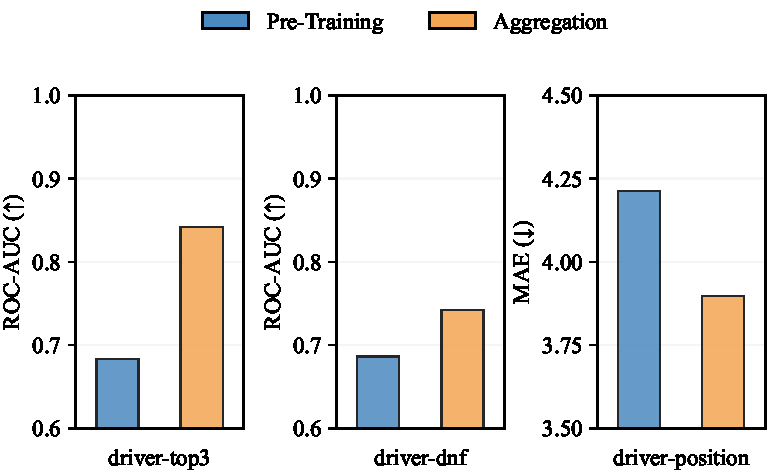
\includegraphics[width=0.88\textwidth]{figures/metartl/12cmp_subplots.pdf}
  \caption{MetaRTL 预训练阶段与聚合阶段的预测表现}
  \label{fig:metartl-stage}
\end{figure}

\section{预训练轮次与规模分析}
\label{sec:metartl-efficiency}

图~\ref{fig:metartl-epochs} 比较不同预训练轮次。
在 \texttt{rel-f1} 的三个任务上，单个 epoch 通常不足以得到较好的
初始表示；五个 epoch 相比一个 epoch 明显改善。
此后曲线并非一致单调：\texttt{driver-top3} 在二十个 epoch
附近也有较高值，而 \texttt{driver-dnf} 与回归任务的最优位置
不同。因此，五轮预训练能够在较少迭代次数下获得较好的初始表示，
但不同任务对应的最优轮次仍存在差异。

\begin{figure}[htbp]
  \centering
  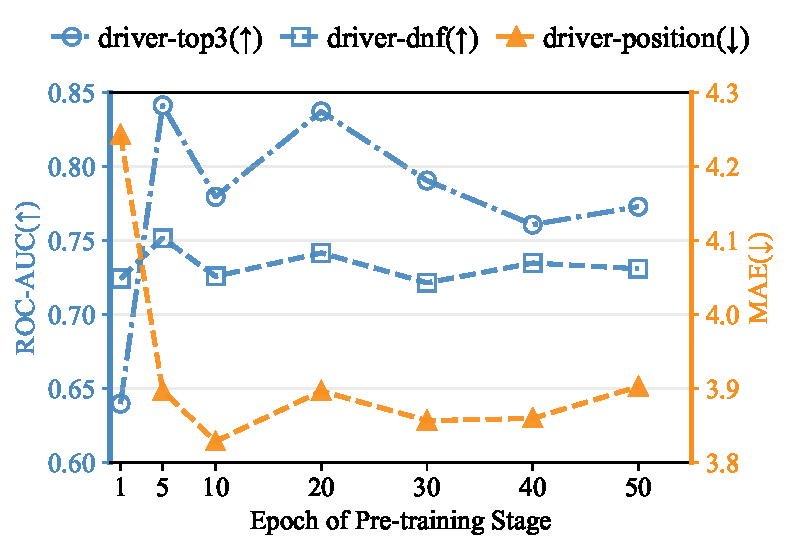
\includegraphics[width=0.78\textwidth]{figures/metartl/k.pdf}
  \caption{不同预训练轮次下的 MetaRTL 表现}
  \label{fig:metartl-epochs}
\end{figure}

为考察模型随图规模变化的运行时间，构造平均出度固定、
目标节点占总节点数 $1\%$ 的合成图，
观察节点数与训练时间的关系。图~\ref{fig:metartl-time}
显示，在该固定出度设置下，总时间随节点数增长大致呈线性趋势；
预训练和聚合两阶段均有不可忽略的时间开销。
在平均出度固定的条件下，该结果表明训练时间随节点规模近似线性增长。
关系模式与路径矩阵稀疏度发生变化时，离线传播矩阵的计算和存储开销
也会随之改变，因此还需结合具体数据库结构分析预计算成本。

\begin{figure}[htbp]
  \centering
  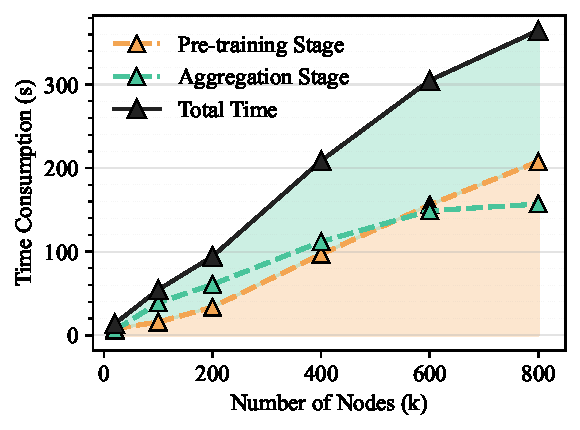
\includegraphics[width=0.78\textwidth]{figures/metartl/time.pdf}
  \caption{固定平均出度的合成图上节点数与训练时间的关系}
  \label{fig:metartl-time}
\end{figure}
